% !TEX Program = lualatex
% class
\documentclass[ngerman]{scrartcl}

% input preamble
\input{../../shared_preamble.tex}
\usepackage{framed}

% manual header
\ihead{Interferometrie}  % inner (left) head
\chead{\textsc{Wachmann} Elias (12004232)\\\textsc{Zach} Andreas (12004790)}  % center head
\ohead{10.03.2023}  % outer (right) head

\addbibresource{Compton.bib}



\begin{document}

%%%%Title Page %%%%
\begin{titlepage}
    \centering
    \includegraphics[width=0.5\textwidth]{../../99_Misc/Logo_KF.pdf}\par\vspace{0.8cm}
    {\scshape\LARGE{Karl-Franzens-Universität Graz}\par}
    {\scshape\LARGE{Institut für Physik}\par}
    \vspace{1cm}
    {\scshape\Large{23S PHY.L02UB Fortgeschrittenenpraktikum 2}\par}
    678 Bachelorstudium Physik, UG2002/2021W\par
    \vspace{1.5cm}
    {\huge\bfseries I. Compton Effekt \& Röntgenfloureszenzanalyse\par}
    \vspace{2cm}
    \begin{table}[H]
        \centering
        \begin{tabular}{c c c}
            \Large Wachmann Elias &  & \Large Zach Andreas \\
            \Large 12004232       &  & \Large 12004790     \\
            \multicolumn{3}{c}{Gruppe 12}
        \end{tabular}
    \end{table}
    \vfill
    \Large Betreut von\par
    Thomas Georg \textsc{Boné}, BSc MSc
    \vfill
    % Bottom of the page
    {\large 17.03.2023\par}
\end{titlepage}
%%%%

\clearpage
\tableofcontents
\newpage

\section[Aufgabenstellung]{Aufgabenstellung \cite{ref:angabe}}
\label{sec:aufgabenstellung}

Der folgende Laborversuch besteht aus vier separaten Teilversuchen, welche sich abermals wie folgt in Unterversuche gliedern:

\begin{itemize}
    \item \textbf{Young'scher Doppelspalt}
          \begin{itemize}
              \item Aufzeichnen des Beugungsmusters von vier Doppelspalten mit unterschiedlichen Spaltbreiten und Spaltabständen % check
              \item Berechnen der Wellenlänge des Lasers % check
              \item Erklären der aufgezeichneten Beugungsmuster durch Vergleich mit theoretisch errechneten Mustern % check
              \item Aufzeichnen des Beugungsmusters eines Liniengitters % check
              \item Bestimmen der Gitterkonstante % check
          \end{itemize}
    \item \textbf{Wellenfront-Analyse / Shearing Interferometer}
          \begin{itemize}
              \item Vermessen des Interferenzmusters % check
              \item Berechnen des Wellenfrontradius % check
          \end{itemize}
    \item \textbf{Polarisation}
          \begin{itemize}
              \item Darstellen der winkelabhängigen Transmission zusammen mit dem theoretischen Verlauf % check
              \item Verifizieren des Gesetzes von Malus % check
              \item Untersuchen des Einflusses des Durchlasswinkels eines weiteren Polarisators zwischen zwei gekreuzten Polarisatoren % check
          \end{itemize}
    \item \textbf{Michelson Interferometer}
          \begin{itemize}
              \item Justieren und generieren von konzentrischen Interferenzmustern % check
              \item Bestimmen der Wellenlänge des Lasers durch Weglängenänderung % check
              \item Untersuchen des absoluten Weglängenunterschieds in den beiden Interferometerarmen sowie Auflösung und Stabilität des Interferometers % check
              \item Justieren und generieren von streifenförmigen Interferenzmustern % check
              \item Untersuchen der Rolle der Polarisation auf die Interfenzfähigkeit des Laserlichts % check
          \end{itemize}
\end{itemize}


\section[Grundlagen]{Grundlagen \cite{ref:angabe}}
\label{sec:grundlagen}


% \begin{figure}[H]
%     \centering
%     \begin{samepage}
%         \includegraphics[width=0.6\linewidth]{fig/Compressed/Angabe_Abb8.png}
%         \caption[Michelson-Interferometer]{Michelson-Interferometer. Strahlengang im Michelson-Interferometer. Ein Laserstrahl aus der Quelle (1) wird am Strahlteiler (2) aufgeteilt, die beiden Teilstrahlen durchlaufen die beiden Interferometerarme der Länge s1 und s2. Nach ihrer Reflexion an den Spiegeln (3,4) werden die Teilstrahlen am Strahlteiler wieder überlagert und interferieren am Beobachtungsschirm (4). \copyright{} Thorlabs, Quelle: \cite{ref:angabe}}
%         \label{fig:michalson_interferometer}
%     \end{samepage}
% \end{figure}




\section{Geräteliste}
\label{sec:geraeteliste}

Für den praktischen Aufbau und die Messungen der geforderten Größen wurden die in \autoref{tab:geraeteliste} aufgelisteten Geräte und Hilfsmittel verwendet.
%
\begin{table}[H]
    \centering
    \begin{samepage}
        \caption[Geräteliste]{Verwendete Geräte und wichtige Materialien}
        \label{tab:geraeteliste}
        \begin{tblrx}{cells={font=\footnotesize}}
            Gerät                     & Hersteller              & Modell               & Messsbereich / Unsicherheit                                                           & Inventar-Nr. \\
            Laser                     & Thorlabs                & CPS532               & $\lambda = \SI{532}{nm}$                                                              & 22442-S01    \\
            diverse Spiegel           & Thorlabs                & KM100                & -                                                                                     & -            \\
            Graufilter                & Thorlabs                & NX1N/M               & -                                                                                     & -            \\
            Doppelspalte              & Phywe                   & 0852300              & -                                                                                     & -            \\
            Gitter                    & Phywe                   & 0852400              & -                                                                                     & -            \\
            Optischer Tisch           & -                       & -                    & -                                                                                     & -            \\
            diverse Halterungen       & Thorlabs                & -                    & -                                                                                     & -            \\
            Sammellinse               & Thorlabs                & FMP1/M               & $f = \SI{40}{mm}$                                                                     & -            \\
            Zerstreuungslinse         & Thorlabs                & FMP1/M               & $f = \SI{-16}{mm}$                                                                    & -            \\
            Shearing-Interferometer   & Thorlabs                & nicht vorhanden      & -                                                                                     & -            \\
            Lichtintensitätsmesser    & Sauter                  & SO 200k              & $\Delta I = (\pm \SI{3}{\percent}\text{rdg} \pm \SI{0.5}{\percent}\text{fs}) \cdot I$ & 51152203     \\
            Polarisationsfolie        & Nitto denko             & -                    & -                                                                                     & -            \\
            Maßband                   & Schuller Eh klar        & Power Tape \SI{3}{m} & Klasse II                                                                             & -            \\
            Michelson Interferometer  & -                       & -                    & -                                                                                     & -            \\
            Rohr                      & -                       & -                    & -                                                                                     & -            \\
            diverse Abbildungsschirme & Wand, Papier, Tür, etc. & -                    & -                                                                                     & -            \\
            Mobiltelefon              & OnePlus                 & 8 Pro                & -                                                                                     & -            \\
        \end{tblrx}
    \end{samepage}
\end{table}
%

\paragraph{Anmerkung zu den Unsicherheiten:} Zur Unsicherheitsangabe werden die jeweiligen Unsicherheitsmaße der Geräte, welche aus den Datenblättern (sofern vorhanden) entnommen werden, verwendet. Für die analogen Messgeräte wird eine kombinierte Ablese- und Messunsicherheit von $\pm\SI{1}{Skalenstrich}$ verwendet.

Alle Teilversuche wurden bei einer Umgebungstemperatur von \SI{24(1)}{\celsius} einem Luftdruck von \SI{1000(10)}{\hecto\pascal} und einer relativen Luftfeuchtigkeit von \SI{33(1)}{\percent} durchgeführt.



\section{Versuchsaufbau}
\label{sec:aufbau}

% \subsection{Young'scher Doppelspalt und Gitter}
% \label{sec:aufbau_doppelspalte_gitter}

% Für den Aufbau zum Versuch \textit{Young'scher Doppelspalt} wird der Laser mittels zwei Spiegel auf das Plättchen mit den vier verschiedenen (siehe \autoref{tab:doppelspalt_abmessungen}) Doppelspalten gelenkt. Der Abstand vom Doppelspalt wird mit \SI{2520(5)}{\milli\meter} bestimmt -- wobei hier noch zur vom Maßband gegebenen Unsicherheit von \SI{1.1}{\milli\meter} eine weitere Unsicherheit durch das Messen in der Luft hinzukommt. Der Aufbau in \autoref{fig:aufbau_doppelspalt} zeigt den optischen Tisch, der Schirm ist rechts im oben angeführten Abstand an der Wand befestigt.
% %
% \begin{figure}[H]
%     \centering
%     \begin{samepage}
%         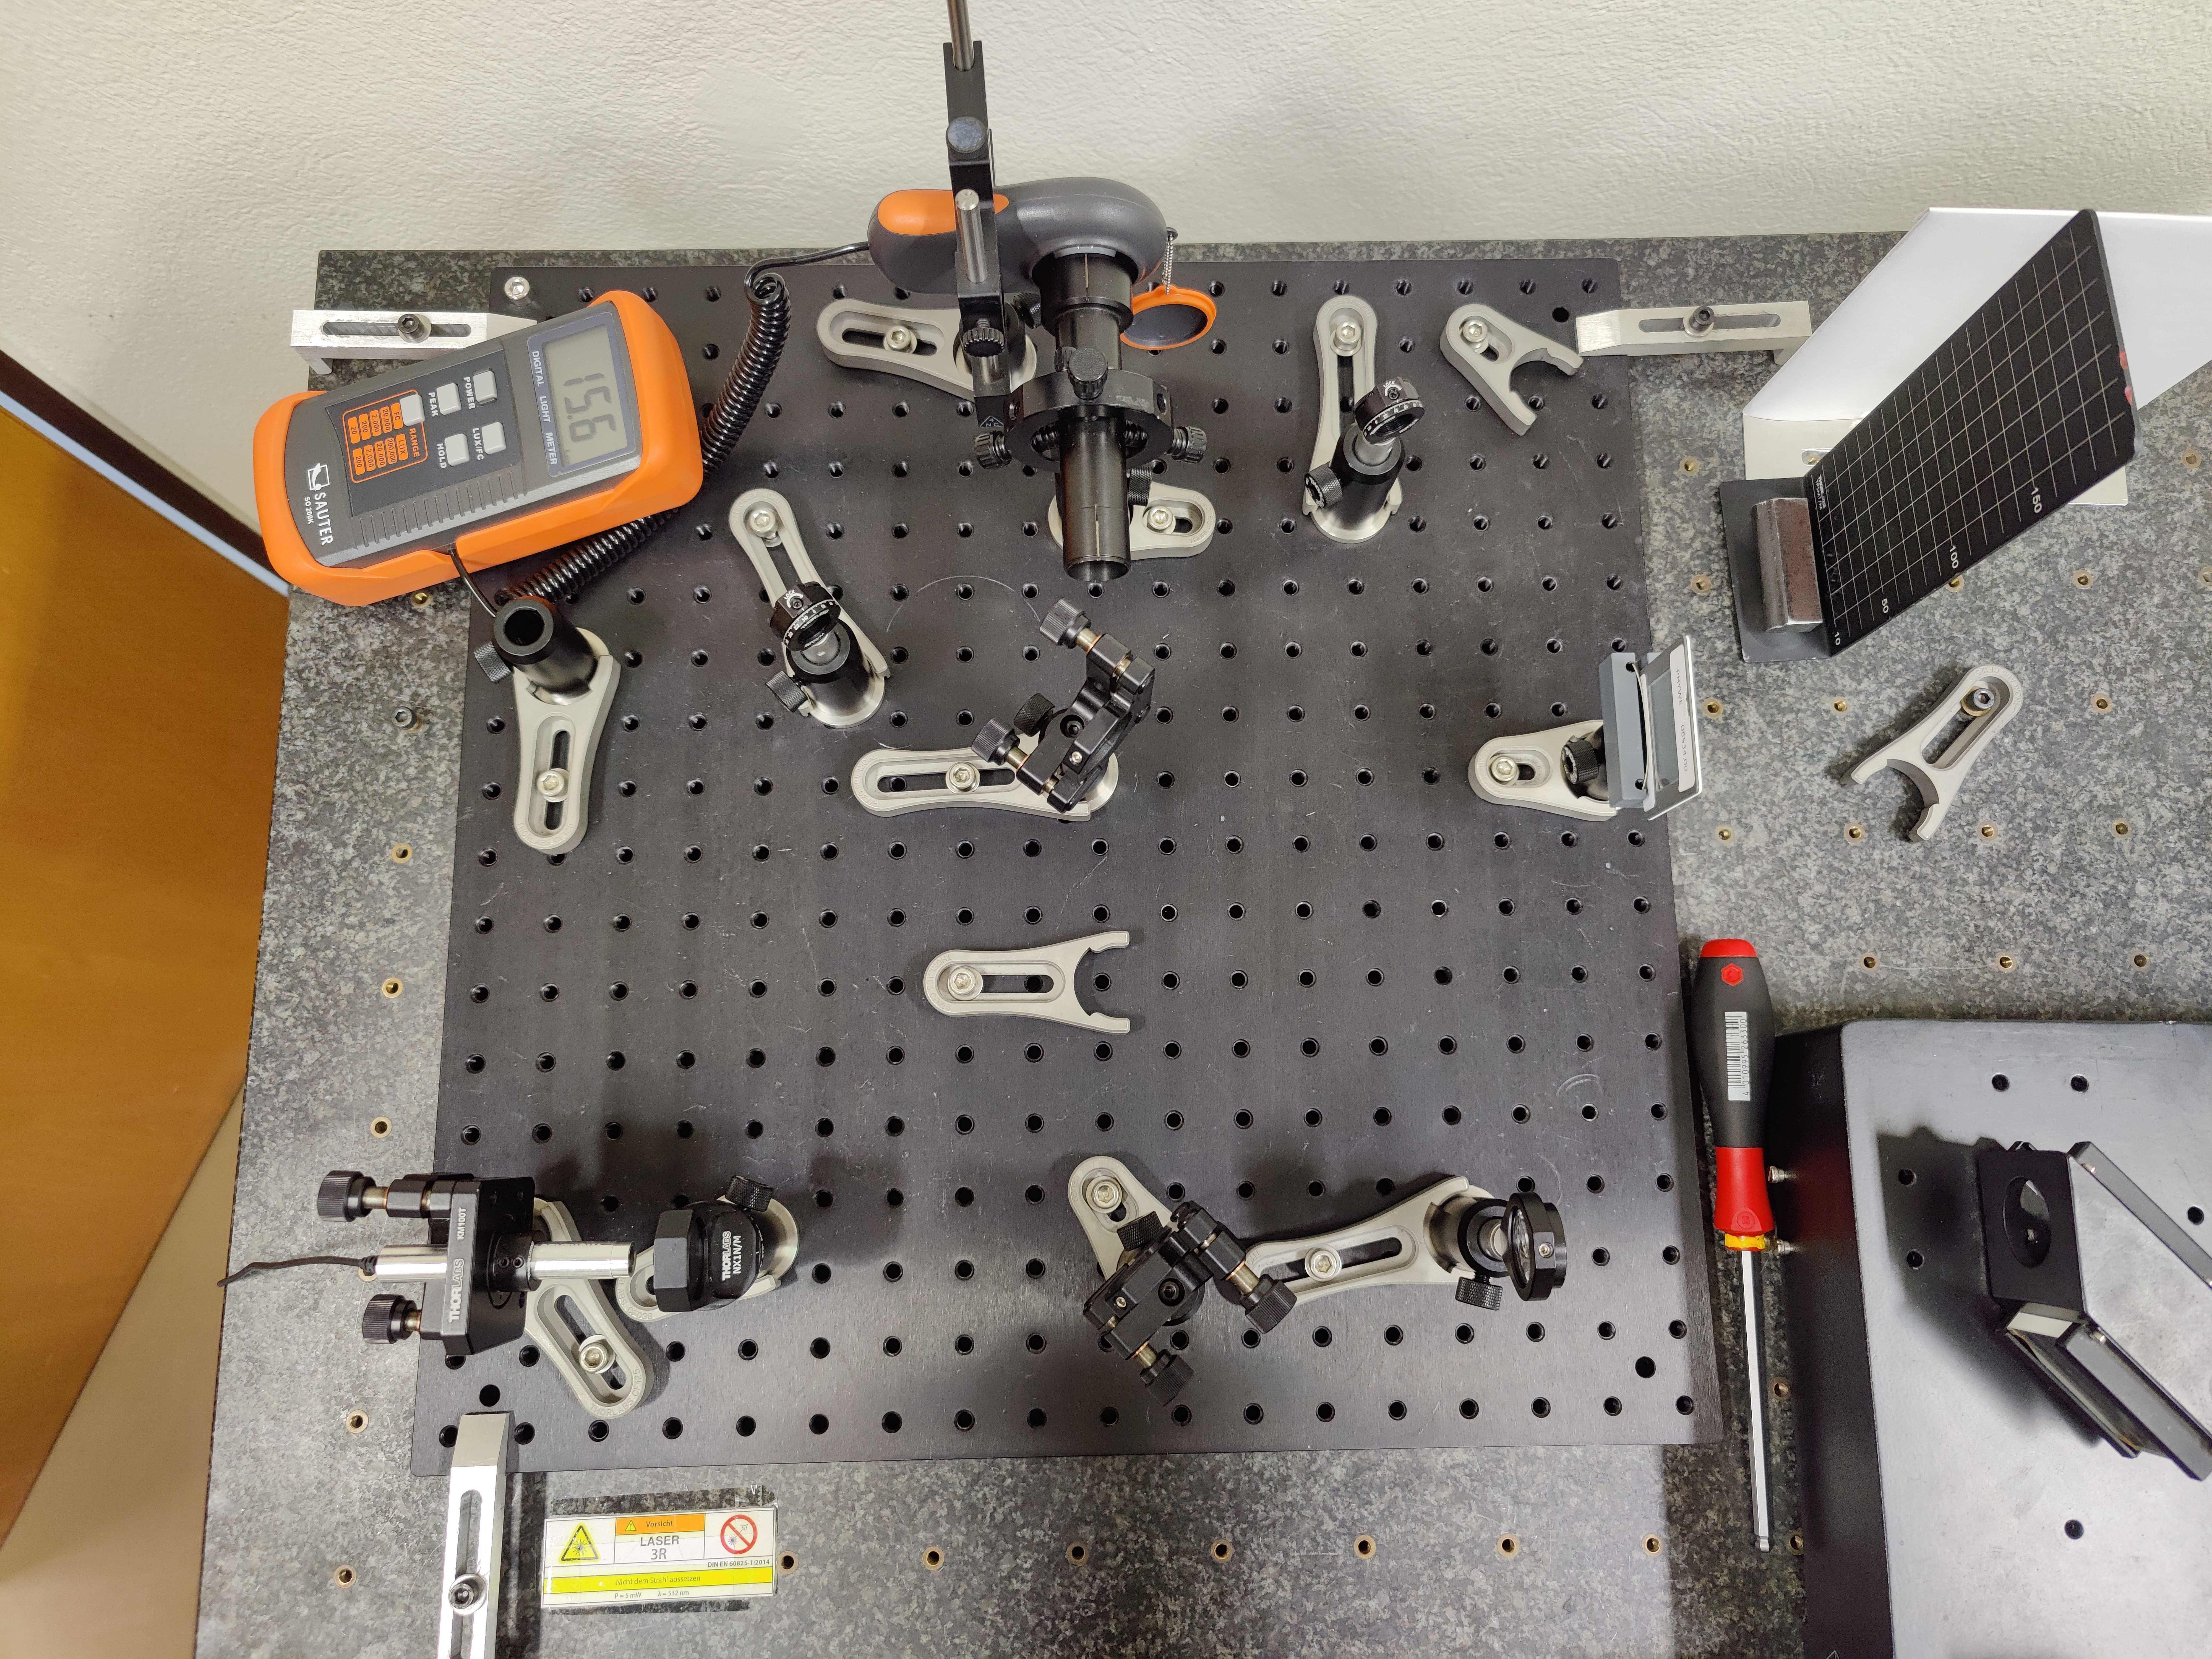
\includegraphics[width=0.7\linewidth]{fig/Compressed/aufbau_doppelspalt.jpg}
%         \caption{Aufbau Young'scher Doppelspalt}
%         \label{fig:aufbau_doppelspalt}
%     \end{samepage}
% \end{figure}

\section{Versuchsdurchführung}
\label{sec:durchfuehrung}

\section{Auswertung}
\label{sec:auswertung}


\section{Diskussion}
\label{sec:diskussion}


\section{Zusammenfassung}
\label{sec:zusammenfassung}


\clearpage
% Literaturverzeichnis
\printbibliography

% Abbildungsverzeichnis
\listoffigures

% Tabellenverzeichnis
\listoftables


\end{document}